\subsection{Robotic setup}
In the experiments repored in this paper we used the robot James 
\ref{figJames}. James is a \textit{upper-torso humanoid robot} with the 
size of about ten years old baby. It has 22 Degrees of Freedom (DOFs) 
actuated by 23 motors. Motors are connected to the joints by belts and 
stainless-steel tendonds. The head is equipped with two eyes, which 
can pan and tilt independently (4 DOFs), and is mounted on a 3-DOF 
neck. The arm has 7 DOFs: three of them are located in the shoulder, 
one in the elbow and three in the wrist. The hand has five fingers 
and is under-actuated with a total of 20 degrees of freedom controlled 
by 8 motors. More details on the platform can be found in \cite{JHRAUW06-12}.

\begin{figure}
\centering
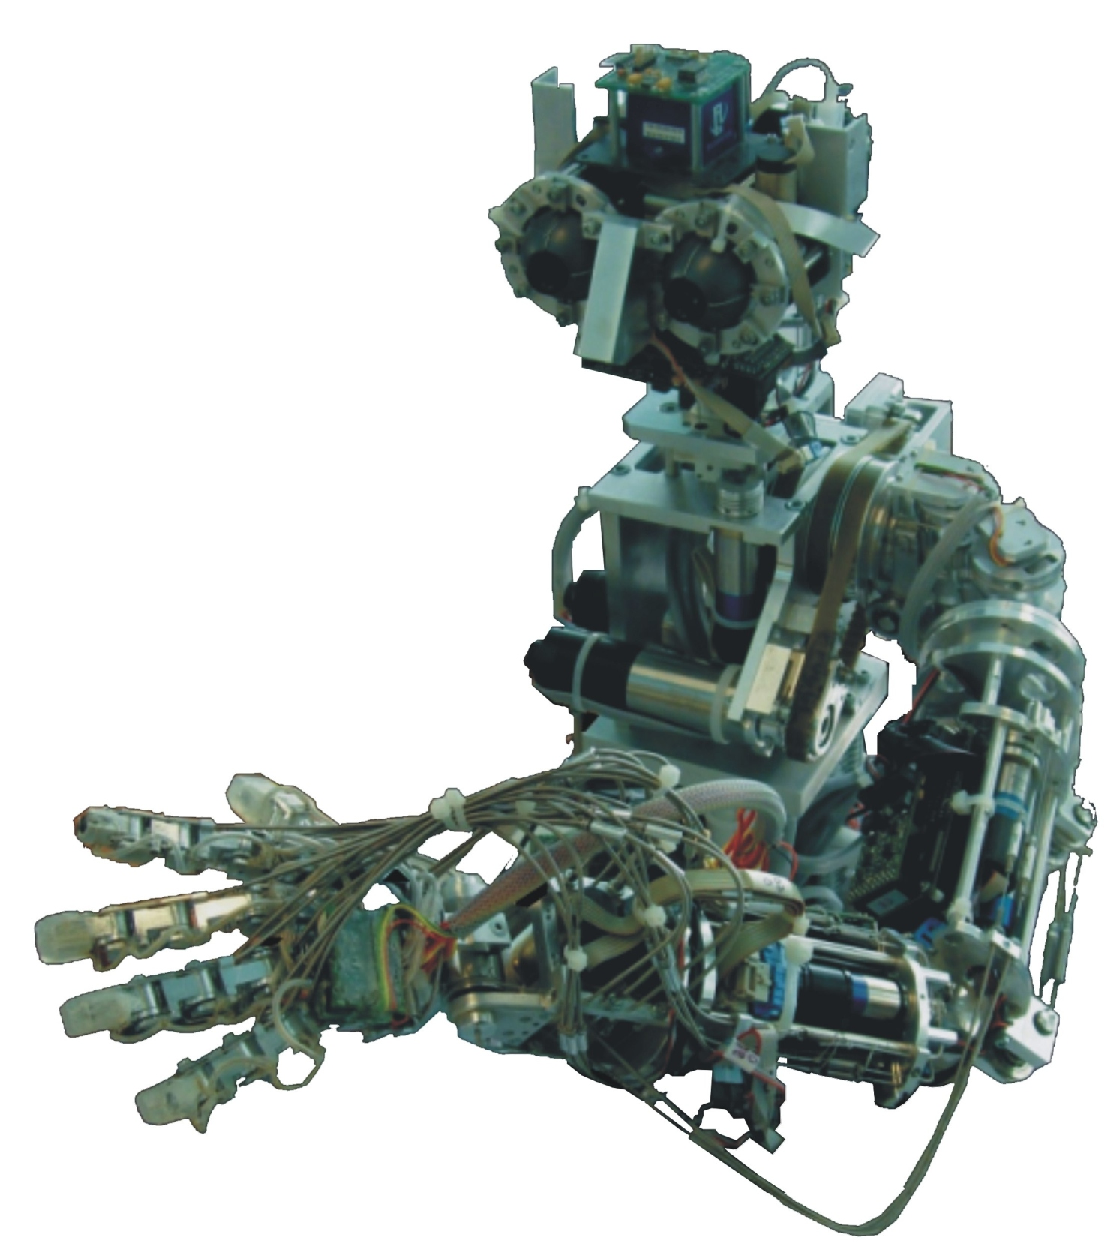
\includegraphics[width=2in]{imgs/james.ps}
\caption{James}
\label{figJames}
\end{figure}
